%!TEX root = main.tex
\section{Introduction}
%Exploring multidiemnsional dataset is hard
\par Visual data exploration is the \emph{de facto} first step in understanding multi-dimensional datasets. This exploration enables analysts to identify trends and patterns, generate and verify hypotheses, and detect outliers and anomalies. However, as datasets grow in size and complexity, visual data exploration becomes challenging. In particular, to identify patterns that merit further investigation, an analyst may need to explore different subsets of the data to determine when and where certain patterns occur. Manually generating and examining each visualization in this space of data subsets (which grows exponentially in number of attributes) presents a major bottleneck.
%Drill-Down for exploration
\begin{figure}[ht!]
% 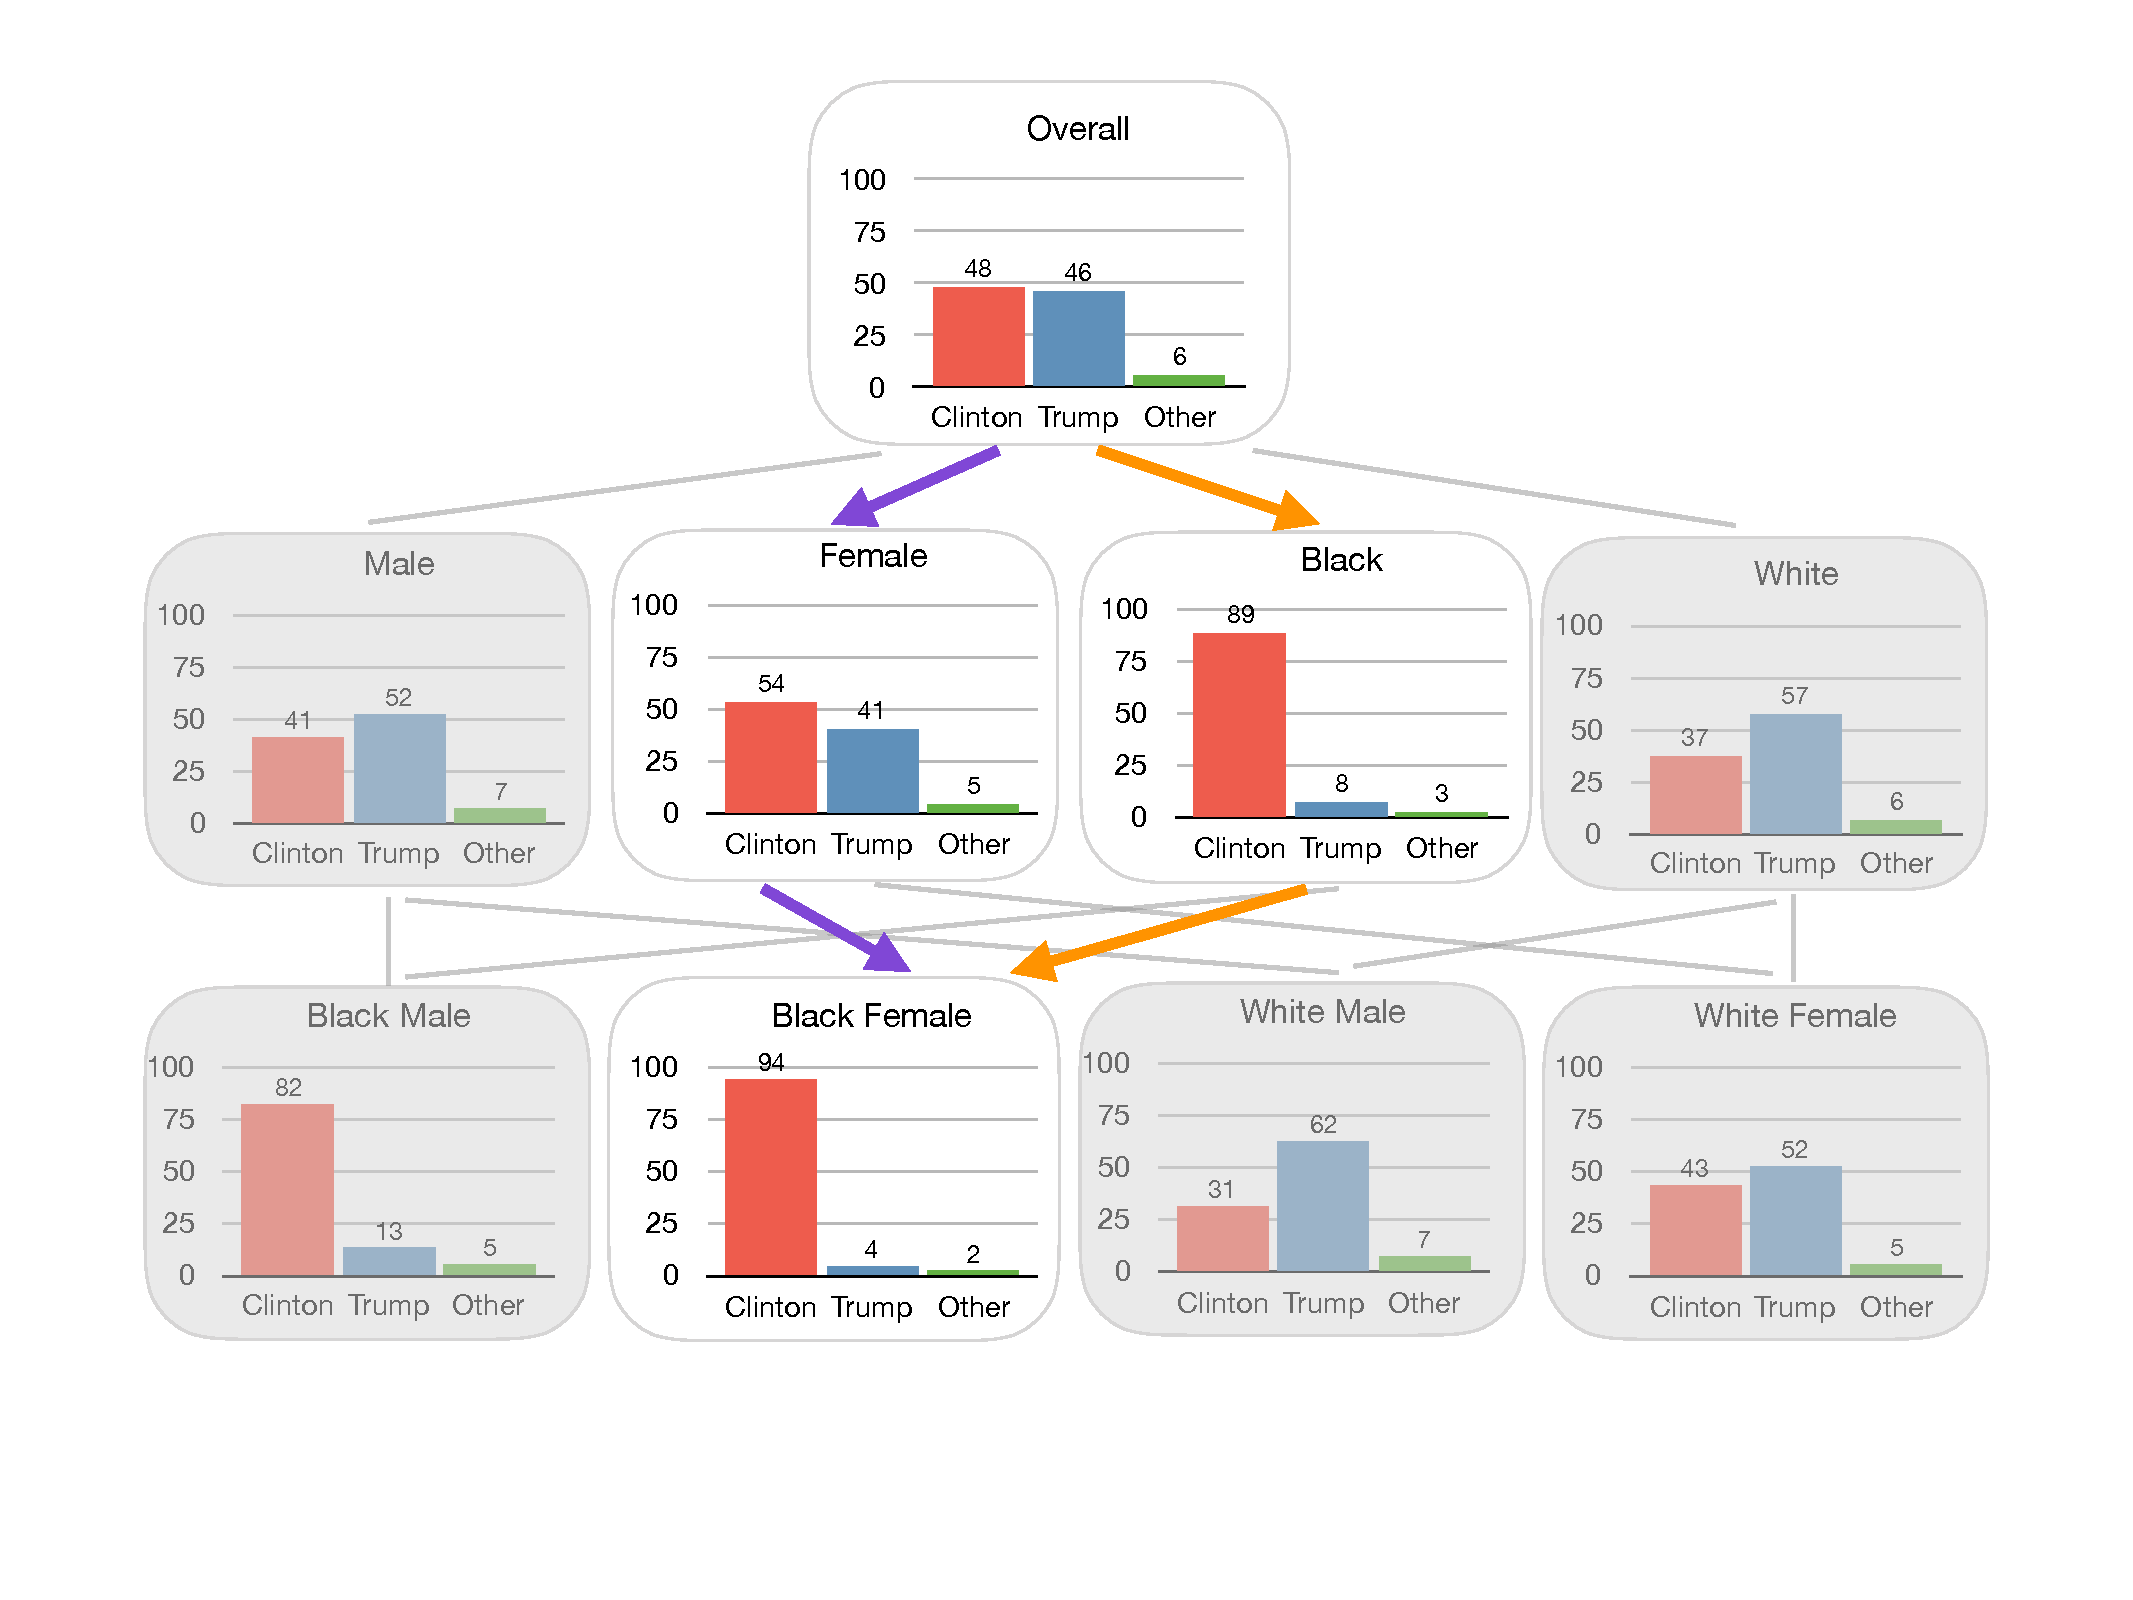
\includegraphics[width=\linewidth]{figures/elections_example_lattice.pdf}
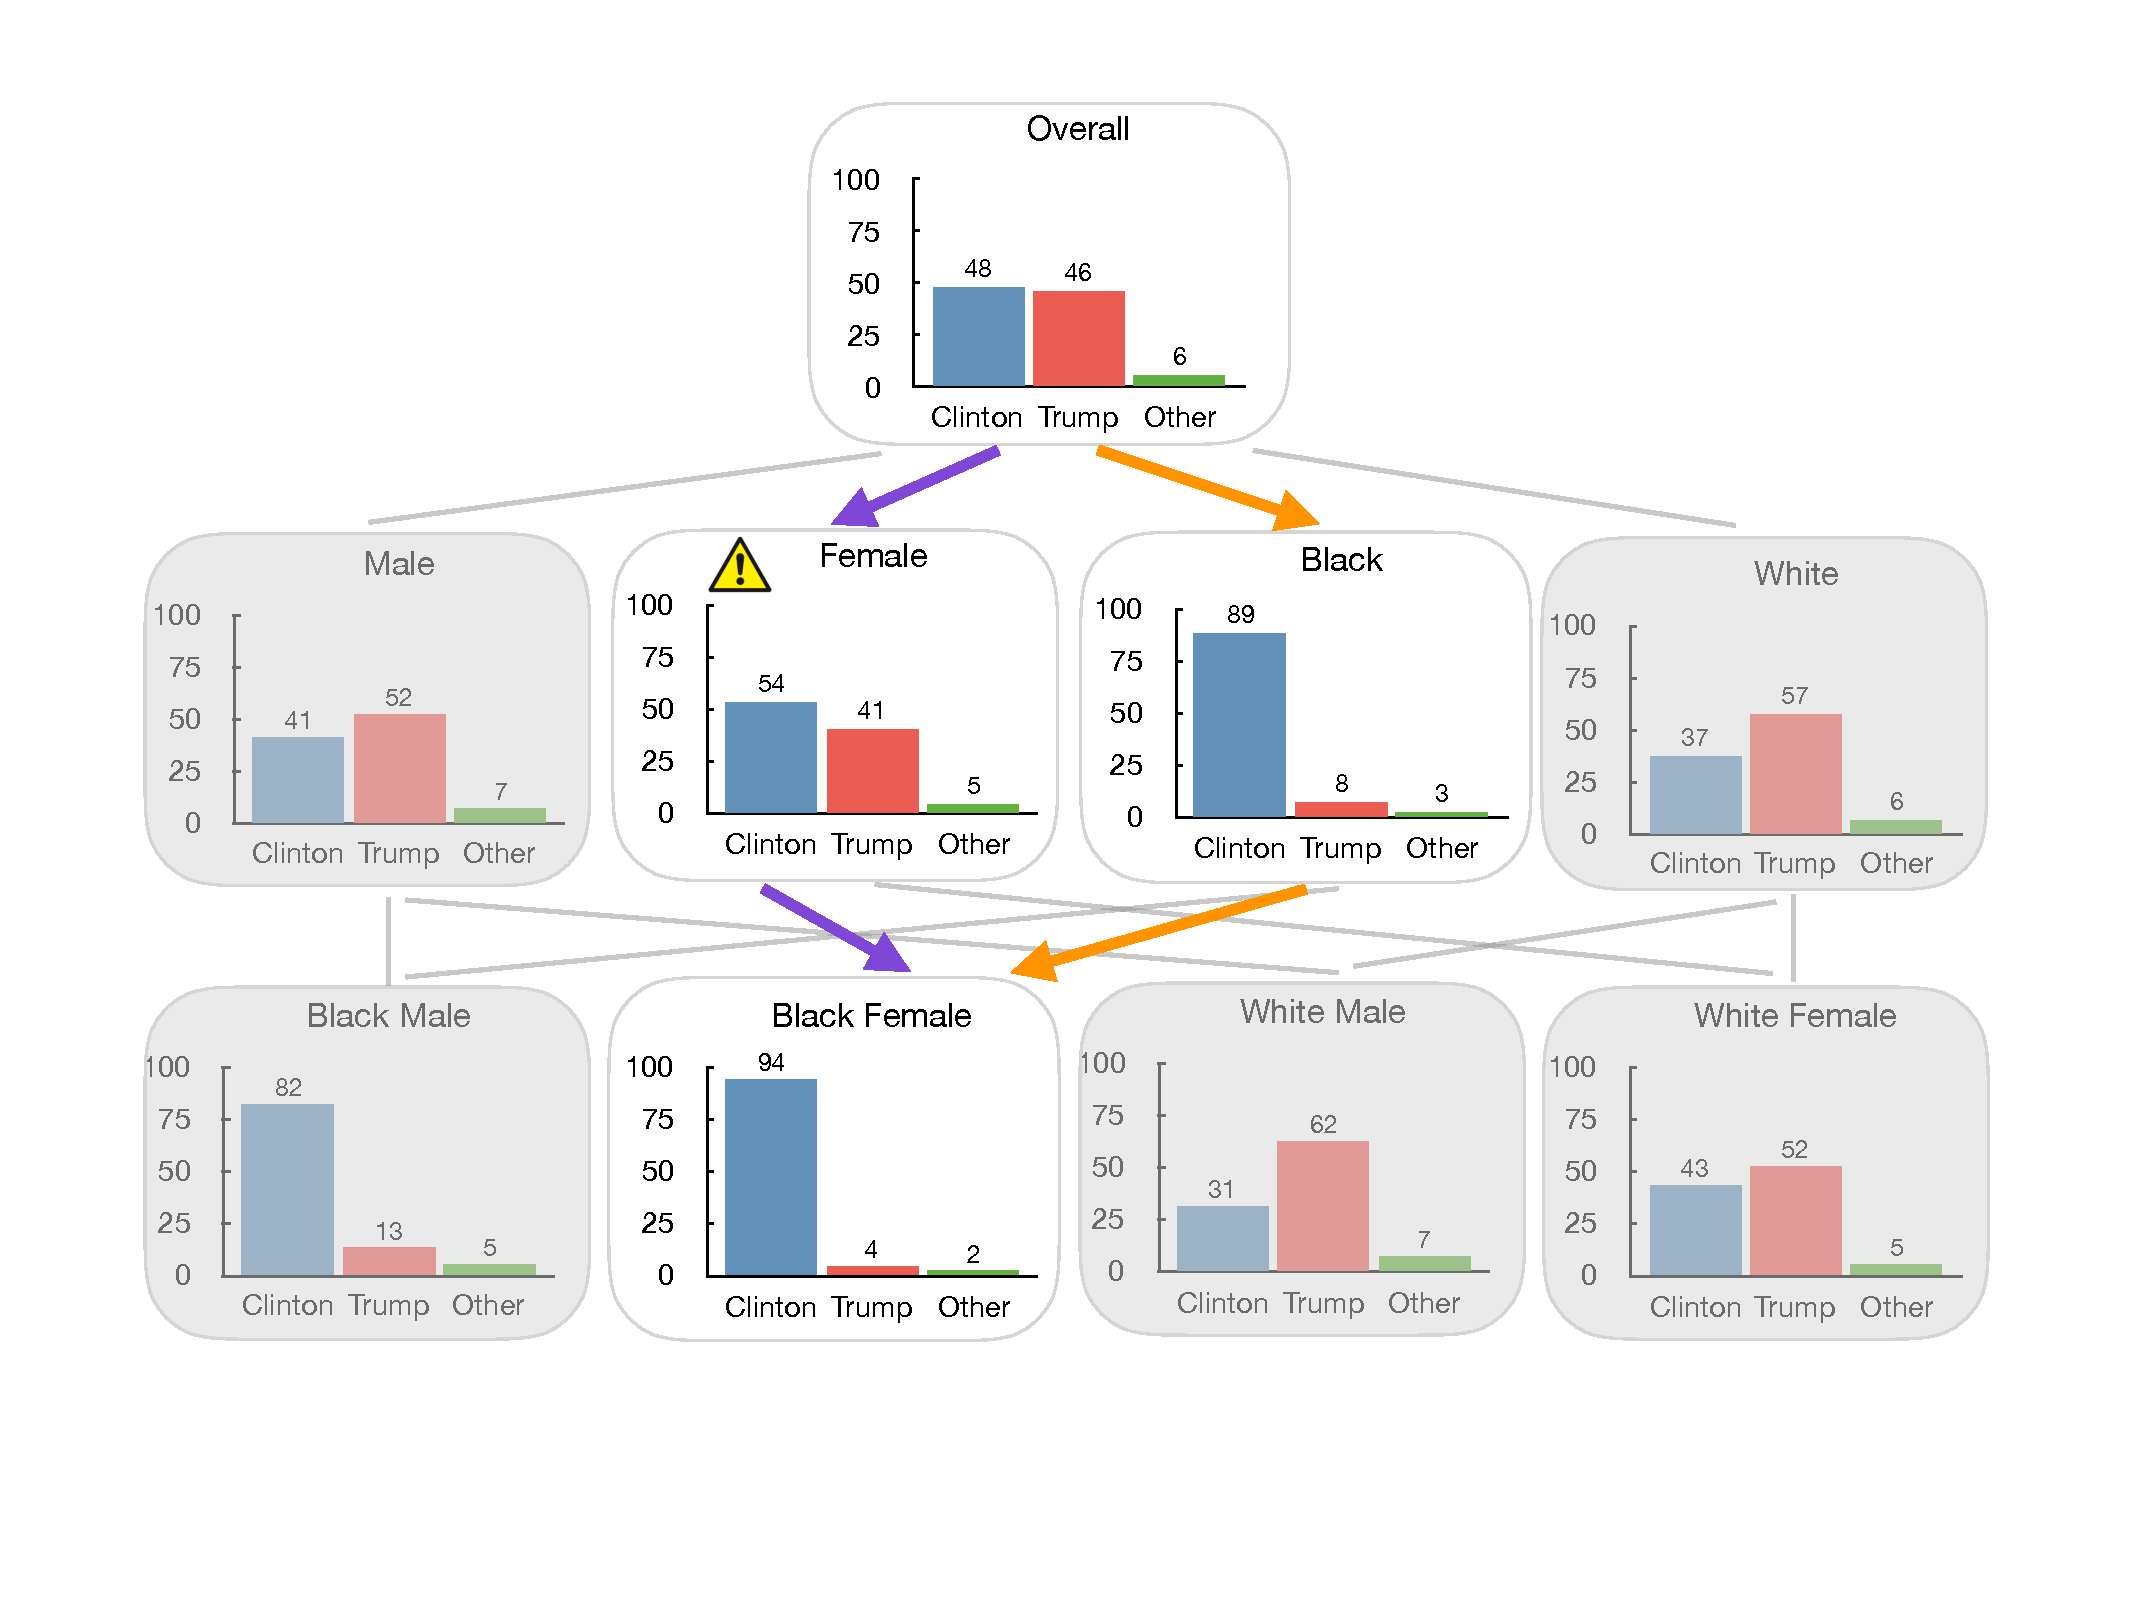
\includegraphics[width=0.95\linewidth]{figures/elections_example_lattice_teaser.pdf}
\caption{Example data subset lattice from the 2016 US election dataset illustrating the drill-down fallacy along the purple path as opposed to the informative orange path.}
\label{fig:elections_example}
\vspace{-10pt}
\end{figure}
\par One way of navigating this combinatorial space is to perform drill-downs on the space of data subsets (hereafter referred to as \emph{lattice}). For example, a campaign manager who is interested in understanding the voting patterns across different demographics (say, race, gender, or social class) using the 2016 US election exit polls~\cite{exitpolls} may first generate a bar chart for the entire population, where the x-axis shows the election candidates and the y-axis the percentage of votes for each of these candidates. In Figure~\ref{fig:elections_example}, the visualization at the top of the lattice corresponds to this overall population. The analyst may then drill down to specific demographics of interest, say gender-based demographics, by generating bar charts for female voters, as shown in the second visualization at the second row of Figure~\ref{fig:elections_example}.
%Challenges associated with drill-down
\par There are three challenges associated with performing manual drill downs in this manner. First, it is often not clear which attributes to drill-down on. Analysts may use their intuition for choosing the drill-down attribute, but such arbitrary exploration may lead to large portions of the lattice being unexplored. Second, an uninformed path taken by analysts may lead to visualizations that are not very surprising or insightful. For example, an analyst may end up wasting effort by drilling down from the \texttt{Black} visualization to the \texttt{Black Female} one in Figure~\ref{fig:elections_example}, since the two distributions are similar and therefore not very surprising. Last but most importantly, an analyst may encounter what we are calling the ``drill-down fallacy''. As shown in Figure~\ref{fig:elections_example}, an analyst can arrive at the \texttt{Black Female} visualization by either going through the purple or the orange drill-down path. An analyst who followed the purple path may be surprised at how drastically the \texttt{Black Female} voting behavior differs from that of the \texttt{Female}. This behavior is no longer surprising if the analyst had gone down the unsurprising orange path that we saw earlier, where the proper reference (i.e., the vote distribution for \texttt{Black}) explains the vote distribution for \texttt{Black Female}. In other words, even though the vote distribution for \texttt{Black Female} is very different from that of \texttt{Female}, the phenomenon can be explained by a more general ``root cause'' attributed to the voting behavior for the \texttt{Black} community. Attributing an overspecific cause to an effect, while ignoring the actual cause, not only leads to less interpretable explanations for the observed visualizations, but can also be detrimental to decision-making. For example, for the campaign manager, this could lead to a misallocation of campaign funds.
\par The aforementioned example demonstrates the \emph{drill-down fallacy}---incomplete insights that result from potentially confounding factors not explored along a drill-down path. In particular, while performing drill-downs on randomly selected paths, analysts may find a ``local difference'' in trends, without being aware of the more ``general phenomenon'' that could explain the trend of interest. Without the proper parent reference visualization that explains the behavior of the visualization of interest, analysts are at risk of falling prey to the drill-down fallacy. A naive solution to avoid this fallacy is to explore all potential drill-down paths. Unfortunately, this approach does not scale with the increasing number of factors in the drill-down path.
\par In this paper, we present a visual data exploration tool, titled \system, that addresses the three aforementioned challenges of exploration through three principles: (i) \textbf{Safety} (i.e., ensure that proper informative references are present to avoid drill-down fallacies), (ii) \textbf{Saliency} (i.e., identify interesting visualizations that convey new information or insights), and (iii) \textbf{Summarization} (i.e., succinctly convey the key insights present in a dataset). To facilitate safety, we develop a notion of \emph{informativeness}---the capability of a reference visualization to explain the visualization of interest. To facilitate saliency, we characterize the notion of \emph{interestingness}---the difference between a visualization and its informative reference in terms of underlying data distribution. Finally, to facilitate summarization, we embrace a \emph{collective} measure of visualization utility by recommending a connected network of visualizations that collectively offer informative insights. Based on these three principles, \system automatically identifies a network of visualizations that succinctly conveys the key informative insights in a dataset. Our user study results demonstrate that \system can guide analysts toward meaningful insights for a variety of tasks. Our contributions include:
\begin{denselist}
\item Identifying and characterizing the notion of ``drill-down fallacy'', a common fallacy that have not yet been studied extensively in the past.
\item Introducing the novel concept of \emph{informativeness} that helps users identify meaningful insights that arise from something \textit{actually interesting} about the data (instead of confounding variables),
\item Designing a system, \system, \change{that automatically identifies} a network of visualizations that succinctly conveys the key informative insights in a dataset,
%that builds a dashboard by
\item Demonstrating the efficacy of our system through a user study evaluation on how well users can retrieve interesting visualizations, judge the importance of attributes, and predict unseen visualizations, against two other summarization baselines.
\end{denselist}
